\section{Statistical Estimators}
\label{chap:algorithms:stat_estimators}

\subsection{Arithmetic mean - Arithmetic weighted mean}
\label{sec:algorithms:robust_mean:mean}

The arithmetic mean of a sample ${x_{1}, x_{2},\dots,x_{N}}$ is
defined as
\begin{equation}
  \label{eq:mean}
  \overline{x}= \frac{1}{N}\sum_{i=1}^{N} x_{i}\,.
\end{equation}
For a random variable $X$ that is normally distributed ($N(\mu,
\sigma)$), the sample mean is the most efficient estimator of the
population mean $\mu$. By the central limit theorem this statement
holds asymptotically for many noise distributions encountered in
practice.

If the noise distribution of $X$ is unknown, its variance can be
estimated from the sample as
\begin{equation}
  \label{eq:mean:sample_variance}
  \hat{\sigma}^{2} = \frac{1}{N-1}\sum_{i=1}^{N}{(x_{i} - \overline{x})^{2}}\,.
\end{equation}
If $X$ has variance $\sigma$ then the average \eqref{eq:mean} has
variance 
\begin{equation}
  \label{eq:mean_variance}
  \sigma_{\mathrm{av}}^{2} = \frac{\sigma^{2}}{N}.
\end{equation}
This relation can be used in place of
Eq.~\eqref{eq:mean:sample_variance} if an \textit{a priori} estimate
of the noise in the images is available and is the same for all images
(homescedastic case).

When each image has its own noise image $\sigma_{i}^{2}(x,y)$
(heteroscedastic case), then the weighted mean
\begin{equation}
  \label{eq:mean_weighted}
  \overline{x} = \left(\sum
    \frac{x_{i}}{\sigma_{i}^{2}} \right)\,\left(\sum
    \frac{1}{\sigma_{i}^{2}}\right)^{-1}
\end{equation}
can be used, giving higher weight to values with lower noise. The
variance of the average value at a given pixel is in this case given
by
\begin{equation}
  \label{eq:average:variance}
  \frac{1}{\sigma_{\mathrm{av}}^{2}} = \sum_{i=1}^{N}\frac{1}{\sigma_{i}^{2}}\,.
\end{equation}

While the average is efficient, it is also sensitive to the presence
of outliers, i.e.~sample values which arise from a process which is
not included in the $N(\mu,\sigma)$ model of the background
noise. Cosmic ray hits and the like that affect single exposures in
the set therefore show up clearly in the stacked image. The average
fails in the presence of a single outlier in the sample.


\subsection{Median}
\label{sec:algorithms:robust_mean:median}

For the computation of the sample median, the sample
$\{x_{i},\,i=1\dots N\}$ is first sorted such that $x_{1} < x_{2} <
\dots < x_{N}$. The median is then the 50th percentile of the ordered
set, i.e.
\begin{equation}
  \label{eq:median_odd}
  x_{\mathrm{med}} = x_{\frac{N+1}{2}} \quad \text{if $N$ is odd}
\end{equation}
and
\begin{equation}
  \label{eq:median_even}
  x_{\mathrm{med}} = \frac{1}{2}(x_{\frac{N}{2}} + x_{\frac{N}{2}+1}) \quad \text{if $N$ is even.}
\end{equation}
This definition for the median for even-sized samples ensures that the
median is an unbiased estimator of the population mean $\mu$ for a
Gaussian error distribution or indeed any distribution that is
symmetric about its mean.

The sample median has a larger variance than the sample average,
i.e.~it is less efficient as an estimator of the population mean. It
is however robust against outliers in the sample since only the central
one or two sample values are actually used for the computation. The
median only fails if half or more of the sample values are outliers,
i.e.~if a given pixel is affected by a cosmic ray hit in half or more
of the images in the stacking list.

\begin{figure}
  \subfigure
  \centering
  \resizebox{0.8\textwidth}{!}{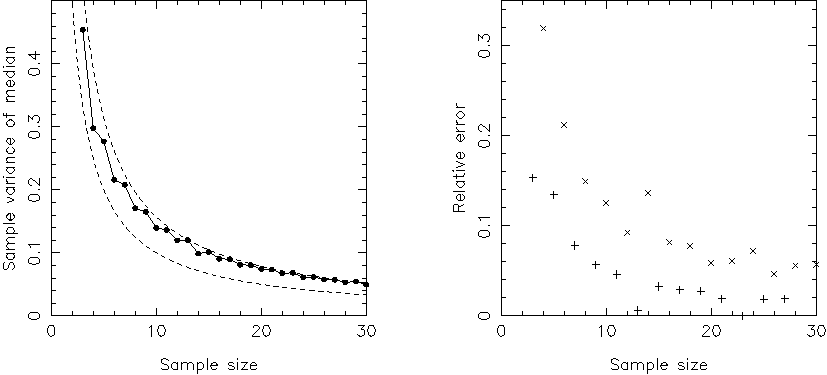
\includegraphics{figures/median_variance}}
  \caption{Sample variance of the median as a function of sample size
    (left panel). The lower dashed curve is the expected variance of
    the arithmetic mean, the upper dashed curve the asymptotic
    variance of the median. The right panel shows the relative error
    compared to the asymptotic variance. Crosses are for even sample
    sizes, pluses for odd sample sizes.}
  \label{fig:median_variance}
\end{figure}

While the sample distribution of the median (which is not Gaussian)
can be written down easily, the computation of its moments and hence
its variance is difficult. A scheme to compute it analytically has
been described in \cite{Maritz-Jarrett1978} and exact values for a few
sample sizes and a number of parent distributions are given in
\cite{Rider1960}. However, these are hardly useful for practical
purposes. The asymptotic value for the ratio of the variances of mean
and median (the \textit{asymptotic relative efficiency} of the median,
\cite{DasGupta2008}) in the Gaussian case is
\begin{equation}
  \label{eq:medvar:asympt}
  \sigma^{2}_{\mathrm{med}} = \frac{\pi}{2}\sigma_{\mathrm{av}}^{2} =
  \frac{\pi\sigma^{2}}{2N}. 
\end{equation}
In Fig.~\ref{fig:median_variance}, we determine the variance of the
median from simulations by drawing for any given sample size $10\,000$
samples from a standard normal distribution. The asymptotic value is
approached from below, which makes it a conservative choice for an
estimate of the median's variance. The relative error, defined as
\begin{equation}
  \label{eq:medvar:asympt:error}
  \frac{\pi/2N - \hat\sigma^{2}_{\mathrm{med}}}{\pi/2N}\,,
\end{equation}
is plotted in the right hand panel of Fig.~\ref{fig:median_variance}. 
For even sample sizes, the relative error is significantly larger than
for odd sizes because the variance is actually lower. For odd-sized
samples, the error is below 10\% for $N\geq7$ ($N\geq 5$
according to \cite{Rider1960}), whereas for even sized samples this
threshold is not crossed until $N\gtrsim 12$. However, as mentioned
above, the asymptotic value in Eq.~(\ref{eq:medvar:asympt}) is
conservative for any $N$ and it is therefore used. 

When each image has its own noise image $\sigma_{i}^{2}(x,y)$
(heteroscedastic case), then a weighted median can be defined as the
point where cumulative weights is equal to $1/2$. Specifically, the
weighted median of an ordered sample of $N$ values $x_{i}$ with
weights $w_{i}$ is 
\begin{align}
  \label{eq:weighted_median}
  x_{\mathrm{wmed}} =
  \begin{cases}
    \displaystyle\frac{x_{j} + x_{j+1}}{2},  &\text{if}\quad
    \sum_{i=1}^{j} w_{i} = 0.5 \\
    \,x_{j},&\text{if}\quad \sum_{i=1}^{j} w_{i} >
    0.5 \quad\text{and}\quad \sum_{i=1}^{j-1} w_{i}< 0.5 
  \end{cases}
\end{align}


\subsection{Kappa-sigma clipping}
\label{sec:algorithms:robust:kappa-sigma}

In the min-max rejection algorithm, a fixed number of sample values
are rejected, regardless whether they can be identified as outliers or
not. If one wants to retain all ``good'' sample values and only reject
true outliers, one has to employ an adaptive method which compares
each sample value to the distribution of the entire sample.

In the $\kappa\sigma$~clipping algorithm, all values that deviate from
the mean by more than $\kappa$ standard deviations are rejected as
outliers. Typically, $\kappa=3$. The mean is usually estimated from
the data, as is the standard deviation if no independent error
estimate is available. One can introduce an iteration which stops once
no more values are rejected. 

Standard $\kappa\sigma$~clipping is not very efficient in removing
low-significance outliers because the estimates of the mean and the
standard deviation are themselves affected by the outliers. Using more
robust estimators of location and scale, like the median and the
inter-quartile range (IQR) or the median absolute deviation (MAD),
improves the situation and makes $\kappa\sigma$~clipping a robust and
easy-to-use adaptive outlier-rejection algorithm. The \HDRL
implementation uses the median and the MAD as robust estimators for
the location and scale.  For a Gaussian distribution, the standard
deviation $\sigma$ is given in terms of the MAD through
\begin{equation}
  \label{eq:sigma-MAD}
  \sigma = \mathrm{MAD} \times 1.4826.
\end{equation}

$\kappa\sigma$~clipping has one parameter, the clipping threshold
$\kappa$. The value of $\kappa$ is not critical if outliers are
expected to lie far from the sample distribution, as is the case for
cosmic ray hits. Weaker effects, such as satellite trails, may require
fine-tuning of $\kappa$.

The functions that make use of $\kappa\sigma$~clipping have a second
parameter, e.g.  \lstinline{niter} which specifies the maximum number
of iterations to run.

The method might fail if more than half of the input images are
affected by outliers at a given pixel because then the estimate of the
MAD might be affected and cause outlier rejection to fail. The method
also requires a sufficient number of input images to be able to obtain
reasonably accurate estimates of the mean and standard deviation.

The variance of the estimator now varies from pixel to pixel depending
on the number of values that are rejected as outliers. Since outliers
are not drawn from the same distribution as the ``good'' data values,
the cleaned sample is equivalent to a smaller sample drawn from the
noise distribution. In the general heteroscedastic case, the variance
is therefore estimated as
\begin{equation}
  \label{eq:ksigma:variance}
  \sigma_{\kappa\sigma}^{2} = \frac{1}{N_{\mathrm{good}}^{2}}
  \sum_{\mathrm{good}} \sigma_{i}^{2}\,.
\end{equation}

\subsection{Mode}
\label{sec:algorithms:robust_mean:mode}

The mode (or modal value) of a distribution of values is defined as
the value of the distribution that appears more often (the maximum of
the function distribution). The \HDRL implements the mode computation
for the case of a discrete distribution.

In the case of a discrete distribution, one can define the ``modal
class'' (the position of the highest peak of the histogram), and the
``modal frequency'' (the value of the highest peak of the histogram),
which are related to the mode of the underlying continuous
distribution.  The value of the modal frequency depends from the
chosen bin size used to create the histogram and from statistical
noise. A large bin size helps in finding a high and unique modal
frequency, but decreases the resolution. A small bin increases the
resolution of the modal class but decreases the modal frequency and
therefore increases the chance that, because of the statistical noise,
the highest peak in the histogram is not related to the mode of the
underlying distribution.

Concerning the determination of the error associated to the mode estimator,
the mode method is special as HDRL
\textbf{calculates the error from the data}
and is not doing pure \textbf{error propagation} as all the
other statistical estimators listed above.
The error calculation depends on the parameter
\verb+error_niter+. If the parameter is set to 0, HDRL estimates the error 
analytically as described below. If the parameter is
larger than 0, the error is calculated by a bootstrap Montecarlo
simulation from the input data with the value of the parameter
specifying the number of simulations. In this case the input data are
perturbed with the bootstrap technique \verb+error_niter+ times and
the mode is derived for each simulation. From this modes the standard
deviation is calculated and returned as error.

The \HDRL implementation in the supported case of discrete
distributions depends on the following parameters:

\begin{itemize}
\item \verb+histo_min+: This parameter defines the lower bound of the
  histogram, i.e. the minimum value of the pixels that are used to
  derive the histogram
  \footnote{\label{footnote1}If $\mbox{histo\_min} < \mbox{histo\_max}+$,
  $\mbox{nbin} = \mbox{floor}(\frac{\mbox{histo\_max}-\mbox{histo\_min}}{\mbox{bin\_size}})+1$,
  data points outside the range [histo\_min,histo\_max] are removed and,
    to be consistent with GSL,  \mbox{histo\_min} is kept to the user value and
  $\mbox{histo\_max} = \mbox{histo\_min} + \mbox{nbin} * \mbox{bin\_size}$}.
    Please note that
  if the lower bound (\verb+histo_min+) is set to the same or to a
  higher value than the upper bound (\verb+histo_max+), both
  parameters are automatically determined from the data by taking the
  minimum value for \verb+histo_min+ and the maximum value for
  \verb+histo_max+.
  \footnote{\label{footnote2}If $\mbox{histo\_min} >= \mbox{histo\_max}$,
  the real minimum internally
  used is always $\mbox{histo\_min} - \frac{\mbox{bin\_size}}{2}$}.

    
\item \verb+histo_max+: This parameter defines the upper bound of the
  histogram, i.e. the maximum value of the pixels that are used to
  derive the histogram\footnoteref{footnote1}.
  Please note that if the upper bound (\verb+histo_max+) is set to the same or
  to a lower value than the lower bound (\verb+histo_min+), both parameters
  are automatically determined from the data by taking the minimum
  value for \verb+histo_min+ and the maximum value for
  \verb+histo_max+
  \footnote{\label{footnote3}If $\mbox{histo\_min} >= \mbox{histo\_max}$,
  the real maximum internally
  used is always $\mbox{histo\_max} + \frac{\mbox{bin\_size}}{2}$}.
\item \verb+bin_size+: This parameter defines the size of the histogram
  bin. Please note that if the value is set to value less or equal to 0, the parameter is
  automatically determined from the data.
\item \verb+mode_method+: This parameter defines the method used to
  compute the mode. Currently there are three methods implemented with an enum:
  \begin{itemize}
  \item \verb+HDRL_MODE_MEDIAN+: This method is the most robust method
    and can/should be used for very asymmetric point
    distributions. For more details see below.
  \item \verb+HDRL_MODE_WEIGHTED+: This method can/should be used with
    asymmetric distributions. For more details see below.
  \item \verb+HDRL_MODE_FIT+: This method give accurate results for
    symmetric distributions but is also more likely to fail. For more
    details see below.
  \end{itemize}
\item \verb+error_niter+: This parameter defines the algorithm to
  compute the error of the mode as, contrary to all the other
  implemented statistical estimators, the mode \textbf{calculates the
    error from the data} and not by \textbf{error
    propagation}. Moreover, it is also special in the sense that one
  can choose between an analytical error estimation and one based on a
  bootstrap simulation. If the parameter is set to 0, HDRL is doing an
  analytical error estimation. If the parameter is larger than 0,
  the error is obtained by a bootstrap Montecarlo simulation from
  the input data with the value of the parameter specifying the number
  of simulations. In this case the input data are perturbed with the
  bootstrap technique and the mode is calculated \verb+error_niter+
  times. From this modes the standard deviation is determined and
  returned as error.
\end{itemize}

In details, the implemented algorithm is performing the following
operations:

\begin{enumerate}
\item Pixels marked as bad (bpm) are removed from the input data.
\item HDRL derives/sets the size of the histogram bins (binsize) as
  follows:
  \begin{itemize}
  \item If \verb+bin_size+ is set to 0, then binsize is automatically
    defined as:
   \[
   {\tt binsize} = 2 \cdot 3.49 \cdot \Sigma /{\tt N_{\rm TOT}}^{1/3}
   \]
   where
   \[
   \Sigma = \biggl\{ \begin{array}{ll}
   
    {\tt MAD}(X)/.67449 & {\rm,  if\ {\tt MAD} (X) \ne 0} \\
      {\tt STDDEV}(X)   & {\rm,  if\ {\tt MAD} (X) = 0} \\
   \end{array}
   \]
   and $N_{\rm TOT}$ is the number of elements of $X$. {\tt MAD} is the
   Median Absolute Deviation and {\tt STDDEV} is the Standard Deviation
   (assuming a degree of freedom of 1). The formula above represents
   Scott's rule for determining the binsize of an histogram, multiplied
   by 2 and with {\tt STDDEV} replaced by {\tt MAD}. The use of the {\tt
     MAD} instead of the standard deviation makes the algorithm more
   robust to the presence of outliers. The factor 1/0.67449 is needed to
   convert {\tt MAD} into standard deviation (this is strictly only valid
   for a Gaussian distribution).
   \item If \verb+bin_size+ is larger than 0, then binsize =
     \verb+bin_size+.
  \end{itemize}
\item Builds a histogram, considering only points in X within {\tt
  max} and {\tt min}. Let's define $v_i$ as the position of the lower
  limits of the i-th bin (a.k.a. ``class'') and $h_i$ as the number of
  elements in the $i-th$ bin (a.k.a. ``frequency''). The vectors $v_i$
  and $h_i$ are outputs, $i$ running from 0 to $N-1$ (do not confuse
  $N$ with $N_{\rm TOT}$).
\item Compute the mode $m$ and its error according to the specified
  algorithm - see
  section~\ref{sec:algorithms:robust_mean:mode_fit},
  section~\ref{sec:algorithms:robust_mean:mode_weighted}, and 
  section~\ref{sec:algorithms:robust_mean:mode_median}
\end{enumerate}

\subsubsection{Mode algorithm: HDRL\_MODE\_FIT}
\label{sec:algorithms:robust_mean:mode_fit}

\begin{enumerate}
\item Locate the highest value of $h$. Define the lower limit of the
  modal class, the value of $v$ that corresponds to $h$, i.e. $v_M$
  with $M$ the index of the highest bin. If there are $N$ adjacent
  bins with the same value of $h$ proceed as follows:
  \begin{enumerate}
    \item Take the mean of the indices of the $n$ bins ($i_1, i_2, ..., i_n$) and round it to the closest integer value $i_m$ and define $M=i_m$.
    \item If there are $n$ non-adjacent bins with the same value of $h$,
      identify the subgroup of $m$ adjacent bins with lower $v$ and
      proceed as before.
    \end{enumerate}
  \item Collect ``at most'' 2 bins below $v_M$, and 2 bins above it. Define $x=[v_{M-2},v_{M-1},v_M,v_{M+1},v_{M+2}]$ and 
$y=[h_{M-2},h_{M-1},h_M,h_{M+1},h_{M+2}]$. If $M\leq 0$ or $M\geq N-3$ be conservative, e.g. if $M=0$ then $x = [v_0,v_1,v_2]$.
\item If there are at least three points in x,y, then fit a parabola,
  otherwise the routine will return with an appropriate error code. Define
  the mode as the value that corresponds to the maximum of the
  parabola.  In formulas, if $p(x)=a_0+a_1x+a_2x^2$ is the equation of
  the parabola ($x$ is continuous variable) and $p(x_M)$ is the
  maximum of the parabola, then the mode is $m = x_M+{\tt binsize}/2$.

  The error on the coefficients of the fit can be used to estimate the
  error on the mode.  The position of the maximum of the parabola is
  $x_M=-a_1/ (2 \cdot a_2)$. Its error can be obtained via error
  propagation:
  %\textcolor{red}{
  \[
    \left( \Delta x_M \right)^2 = \left( \frac{\Delta a_1}{2a_2} \right)^2 +\left( \frac{a_1 \Delta a_2}{2a_2^2} \right)^2 + {\rm COVAR\_TERM}
  \]
  COVAR\_TERM is ad additional term due to the fact that variables $a_2$ and $a_1$ are not independent:
  \[
    {\rm COVAR\_TERM} =  2\cdot \frac{-1}{2\cdot a_2} \frac{a_1}{2a_2^2} \cdot Covar(a_2,a_1)
  \]
  $Covar(a_2,a_1)$ is the term of the covariance matrix. The covariance matrix is defined as the inverse of the following matrix (parabolic case):
\[
  \begin{bmatrix}
    \sum w_i        &   \sum w_i x_i    &  \sum w_i  x_i^2 \\
    \sum w_i x_i    &   \sum w_i x_i^2  &  \sum w_i  x_i^3 \\
    \sum w_i x_i^2  &   \sum w_i x_i^3  &  \sum w_i  x_i^4 
  \end{bmatrix}
  \]
  Because we do not consider the errors on the individual points, we can set $w_i = 1$. HDRL actually uses GSL to compute the fit coefficients $a_{i}$, and the associated errors (taking into account of the covariance). 
  %}

\item If the fit does not converge, or the  mode $m$ computed above is more
  than {\tt binsize}/2 outside the maximum bin, HDRL exit with corresponding
  error message.
  In formulas, if
  \[
  \left| v_M+{\tt binsize}/2-m \right| >{\tt binsize}
  \]
  HDRL issues an appropriate error message.
\end{enumerate}


\begin{figure}
\begin{center}\subfigure
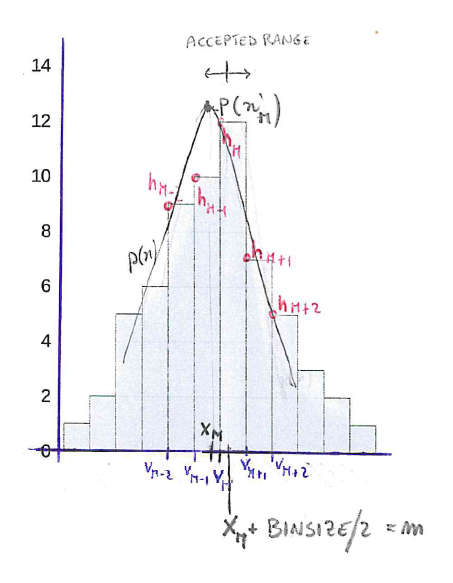
\includegraphics[width=0.4\textwidth]{figures/mode_fig1.jpg}
\caption{Graphic representation of the ``fit'' method to compute the mode of an histogram.}
\label{fig:fit}
\end{center}
\end{figure}
Figure \ref{fig:fit} illustrates the method.


\subsubsection{Mode algorithm: HDRL\_MODE\_WEIGHTED}
\label{sec:algorithms:robust_mean:mode_weighted}

\begin{enumerate}
\item Locate the highest value of $h$. Define the lower limit of the
  modal class, the value of $v$ that corresponds to $h$, i.e. $v_M$ with $M$ the index of the highest bin. If
  there are $N$ adjacent  bins with the same value of $h$ proceed as follows:
  \begin{enumerate}
    \item Take the mean of the indices of the $n$ bins ($i_1, i_2, ..., i_n$) and round it to the closest integer value $i_m$ and define $M=i_m$.
    \item If there are $n$ non-adjacent bins with the same value of $h$,
      identify the subgroup of $m$ adjacent bins with lower $v$ and
      proceed as before.
    \end{enumerate}
 \item If $n$ is even, define  $v'=v_M-{\tt binsize}/2$, if $n$ is odd define $v'=v_M$.

 \item Collect one bin before ($h_0$) and one after ($h_2$) the group
   of $n$ bins with highest value; in formulas
   $v_{M-1-{\rm int}(n/2)}$,$v_{M+1+{\rm int}(n/2)}$, where
   ${\rm int}(n/2)$ is the integer part (if $n=3$ then
   ${\rm int}(n/2)=1$) . Define $f0=h_0$ and $f2=h_2$. If $M=0$ then
$f0=0$. If $M=N-1$ then $f2=0$.

  
 \item Define $d1 = f1-f0$, $d2 =f1-f2 $ and the weight $w=d1/(d1+d2)$.
 \item Define the mode $m=v_M+{\tt binsize}\cdot w$. If $w=0$ or infinite,
   then set $w=0.5$.

  Error on the mode is computed via error propagation, assuming that the errors on d1 and d2 are given by Poisson statistics ($\Delta f_i = \sqrt{f_i}$)
  \begin{eqnarray}
  \Delta d_1 &=& \sqrt{f1+f0} \nonumber \\
  \Delta d_2 &=& \sqrt{f1+f2} \nonumber \\
    \Delta m &=& {\tt binsize}\cdot \Delta w \nonumber \\
\Delta w^2 &=& \left( \frac{d_2\Delta d_1}{(d_1+d_2)^2} \right)^2 + \left( \frac{d_1 \Delta d_2}{(d_1+d_2)^2}\right)^2 
  \end{eqnarray}

\end{enumerate}
Figure \ref{fig:weight} illustrates the method with $n$=1,2, and 3.

\begin{figure}
\begin{center}\subfigure
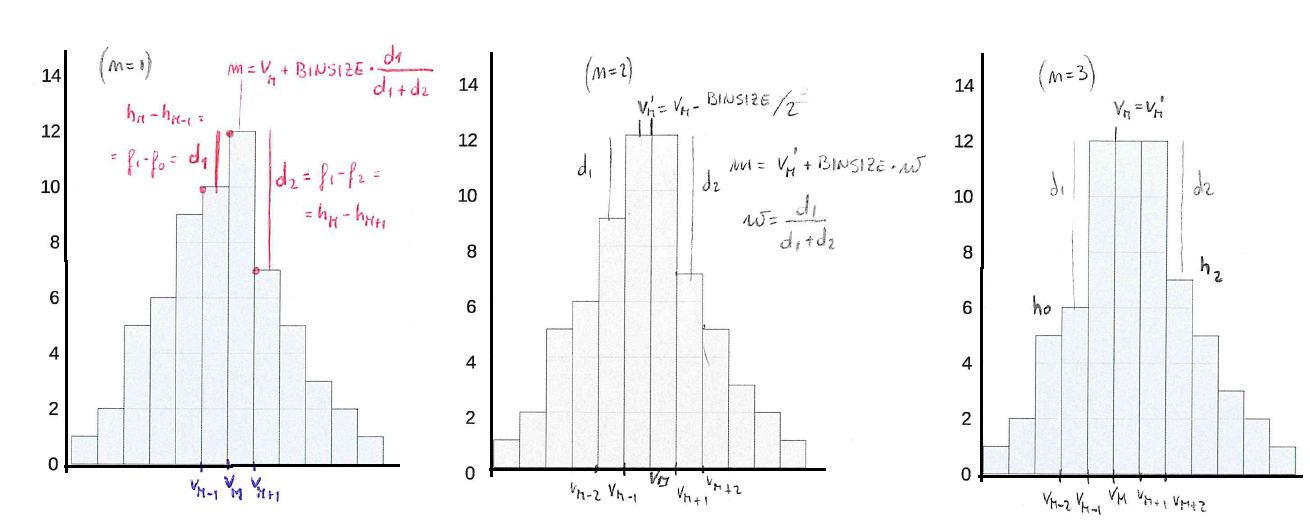
\includegraphics[width=1.05\textwidth]{figures/mode_fig2.jpg}
\caption{Graphic representation of the ``weight'' method to compute
  the mode of an histogram. Three cases are show: single modal class
  (n=1, left panel), two modal classes (n=2, central panel), and three
  modal classes (n=3, right panel).}
\label{fig:weight}
\end{center}
\end{figure}
\subsubsection{Mode algorithm: HDRL\_MODE\_MEDIAN}  
\label{sec:algorithms:robust_mean:mode_median}

This algorithm is suited
for strongly asymmetric distributions (as Gamma distributions).
\begin{enumerate}


\item Locate the highest value of $h$. Define the lower limit of the
  modal class, the value of $v$ that corresponds to $h$, i.e. $v_M$ with $M$ the index of the highest bin. If
  there are $N$ adjacent  bins with the same value of $h$ proceed as follows:
  \begin{enumerate}
    \item Take the mean of the indices of the $n$ bins ($i_1, i_2, ..., i_n$) and round it to the closest integer value $i_m$ and define $M=i_m$.
    \item If there are $n$ non-adjacent bins with the same value of $h$,
      identify the subgroup of $m$ adjacent bins with lower $v$ and
      proceed as before.
    \end{enumerate}

  \item Define the mode as the median of the values of
    $v_M< X <v_M+binsize$. The error on the median is the standard
    deviation of the $X$ values.
    %\textcolor{red}{standard deviation of the $X$ values}.
\end{enumerate}
